\documentclass[a4paper,14pt]{extreport}
\usepackage[left=1.5cm,right=1.5cm,
    top=1.5cm,bottom=2cm,bindingoffset=0cm]{geometry}
\usepackage{scrextend}
\usepackage[T1,T2A]{fontenc}
\usepackage[utf8]{inputenc}
\usepackage[english,russian,ukrainian]{babel}
\usepackage{tabularx}
\usepackage{amssymb}
\usepackage{color}
\usepackage{amsmath}
\usepackage{mathrsfs}
\usepackage{listings}
\usepackage{graphicx}
\graphicspath{ {./images/} }
\usepackage{lipsum}
\usepackage{xcolor}
\usepackage{hyperref}

\usepackage{tcolorbox}
\usepackage{tikz}
\usepackage[framemethod=TikZ]{mdframed}
\usepackage{wrapfig,boxedminipage,lipsum}
\mdfdefinestyle{MyFrame}{%
linecolor=blue,outerlinewidth=2pt,roundcorner=20pt,innertopmargin=\baselineskip,innerbottommargin=\baselineskip,innerrightmargin=20pt,innerleftmargin=20pt,backgroundcolor=gray!50!white}
 \usepackage{csvsimple}
 \usepackage{supertabular}
\usepackage{pdflscape}
\usepackage{fancyvrb}
%\usepackage{comment}
\definecolor{ggreen}{rgb}{0.,1,0}
\definecolor{rred}{rgb}{1,0.1,0.1}
\usepackage{array,tabularx}
\usepackage{colortbl}

\usepackage{varwidth}
\tcbuselibrary{skins}
\usepackage{fancybox}




\usepackage{float}
\usepackage{wrapfig}
\usepackage{framed}





\begin{document}
\renewcommand{\bibname}{Список використаної літератури}
\pagecolor{white}
\begin{titlepage}
  \begin{center}
    \large
    Національний технічний університет України \\ "Київський політехнічний інститут імені Ігоря Сікорського"


    Факультет Електроніки

    Кафедра мікроелектроніки
    \vfill

    \textsc{ЗВІТ}\\

    {\Large   Про виконання лабораторної роботи №7\\
      з дисципліни: «Твердотільна електроніки-1»\\[1cm]

      Дослiдження вольт-амперних характеристик
      бiполярних транзисторiв

    }
  \bigskip
\end{center}
\vfill

\newlength{\ML}
\settowidth{\ML}{«\underline{\hspace{0.4cm}}» \underline{\hspace{2cm}}}
\hfill
\begin{minipage}{1\textwidth}
Виконавець:\\
Студентка 3-го курсу \hspace{4cm} $\underset{\text{(підпис)}}{\underline{\hspace{0.2\textwidth}}}$  \hspace{1cm}Д.\,О.~Заєць\\
\vspace{1cm}

Перевірив: \hspace{6.1cm} $\underset{\text{(підпис)}}{\underline{\hspace{0.2\textwidth}}}$  \hspace{1cm}Л.\,М.~Королевич\\

\end{minipage}

\vfill

\begin{center}
2020
\end{center}
\end{titlepage}
%---------------------------------------------------------------------------------------------------------------------------------------------------------------------------------



\begin{center}МЕТА РОБОТИ\\ \end{center}

Теоретичне вивчення і практичне дослідження біполярних транзисторів з допомогою вимірювання вольт-амперних характеристик, визначення фізичних та основних технічних параметрів біполярних транзисторів із вольт-амперних характеристик.

\begin{center} ЗАВДАННЯ\\ \end{center}

1. Вивчити структуру паспортних параметрів біполярних транзисторів. Ознайомитися із
вимірювальним стендом та використовуваними приладами (рис. 1, 2, 3, 4).\par
2. Зібрати схему для дослідження вольт-амперних характеристик біполярних транзистора
ввімкненого за схемою із спільним емітером (або із спільною базою).\par
3. Визначити експериментально і побудувати графічно сімейство вхідних характеристик
транзистора - залежність вхідного струму від вхідної напруги.\par
4. Визначити експериментально та побудувати графічно сімейство вихідних характеристик
транзистора - залежність вихідного струму від вихідної напруги.\par
5. * Провести температурні дослідження ВАХ біполярного транзистора при підвищеній
температурі $T_2 \approx$+70 °С.\par
6. **Із вхідних та вихідних ВАХ побудувати характеристики зворотного зв'язку і прямої
передачі.\par
7. За побудованими графіками характеристик визначити основні параметри біполярного
транзистора: коефіцієнт підсилення струму бази - $\beta$; коефіцієнт підсилення струму емітера - $\alpha$; диференційні опори емітерного $r_e$ і колекторного $r_c$ переходів для вибраної робочої точки $A_p(I_c, U_{ce})$; графічно визначити дифузійний потенціал емітерного переходу $\varphi_{0e}$ та опір бази $r_b$.\par
8. Провести аналіз результатів досліджень, і зробити висновки з виконаної роботи.\par


\newpage
\begin{center}СХЕМА ВИМІРЮВАННЯ\\ \end{center}
\begin{figure}[h]
\center{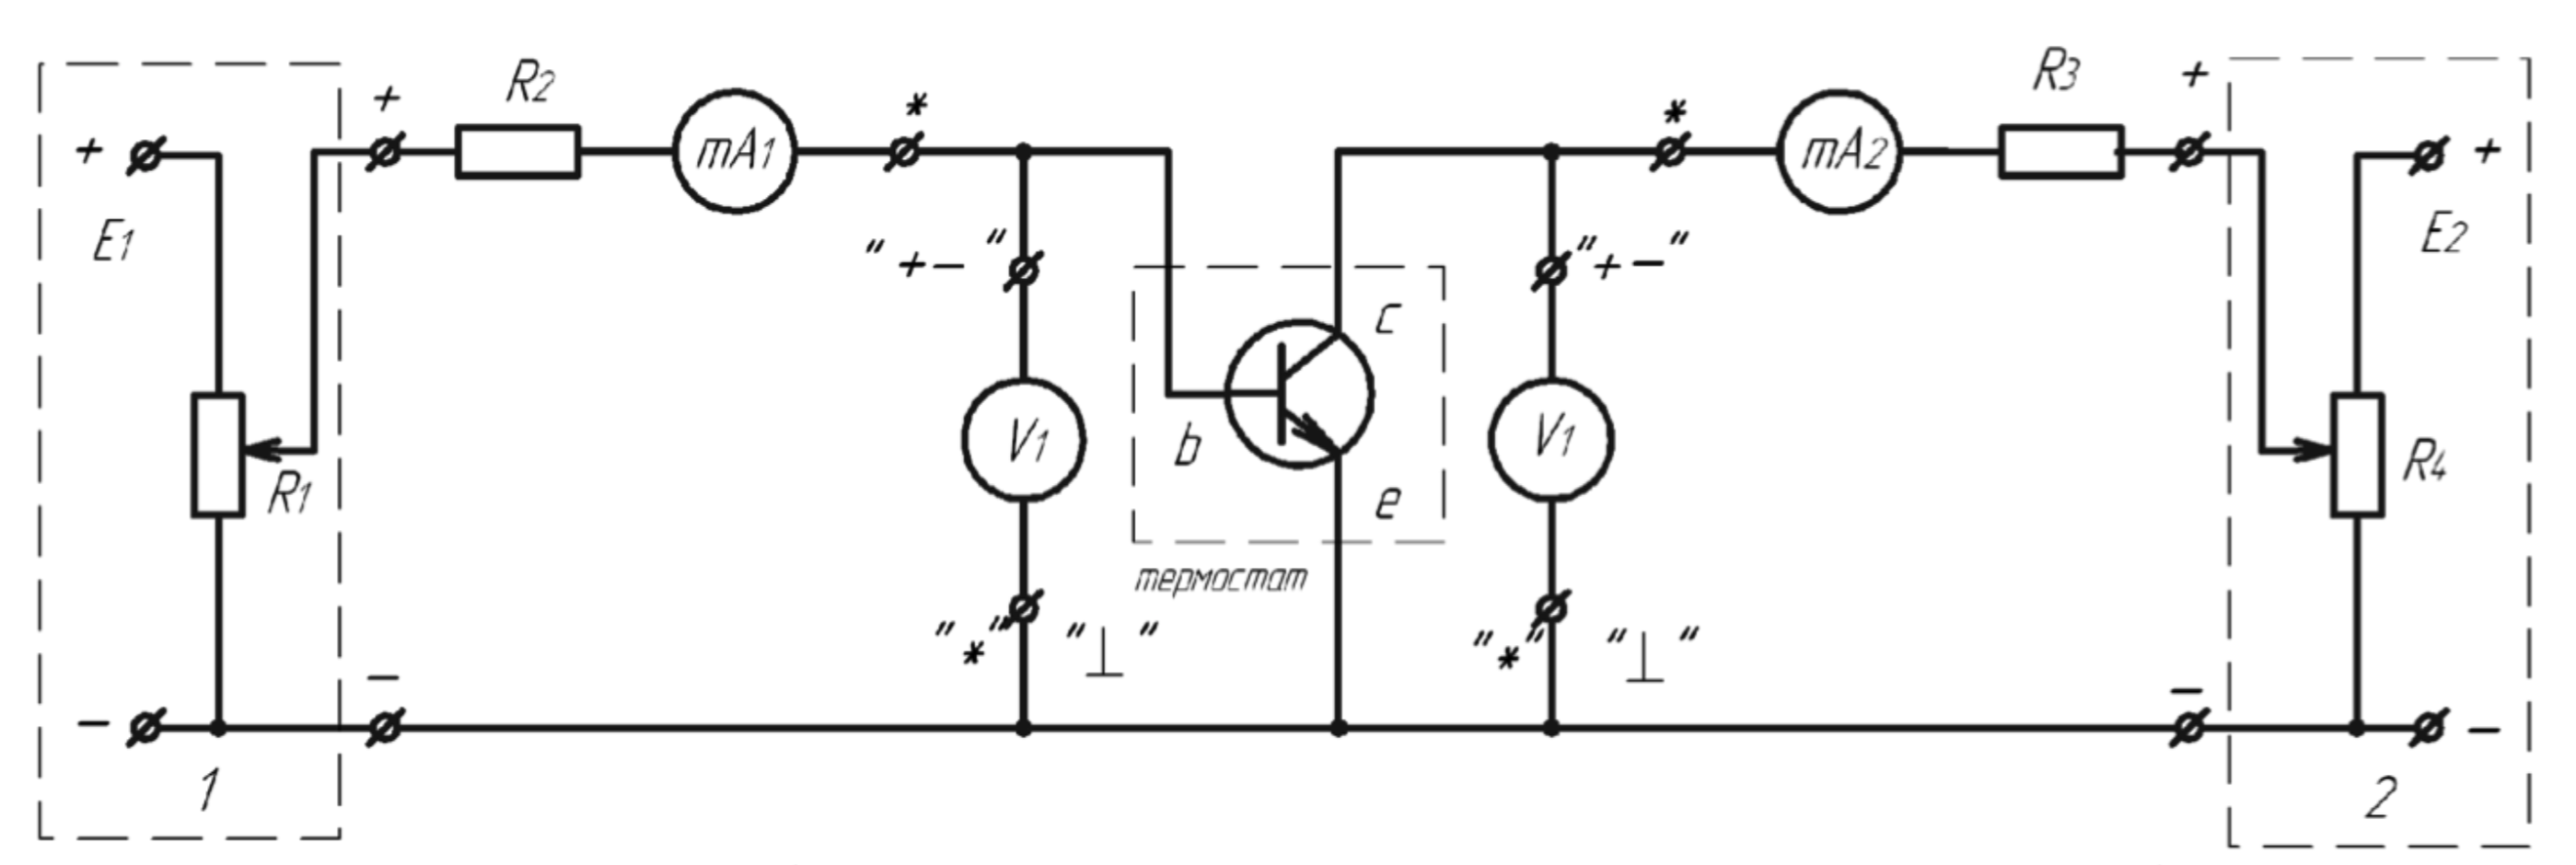
\includegraphics[width=1\linewidth]{1.1.png}}
\caption{Схема для дослідження вольт – амперних характеристик транзистора ввімкненого за схемою зі спільним емітером.}
\label{ris:image01}
\end{figure}

%---------------------------------------------------------------------------------------------------------------------------------------------------------------------------------












%1---------------------------------------------------------------------------------------------------------------------------------------------------------------------------------
\clearpage
\newpage
\begin{center}ТАБЛИЦІ З ВХІДНИМИ ПАРАМЕТРАМИ\\ \end{center}
\vspace{0.5 cm}
\begin{figure}[h]
\center{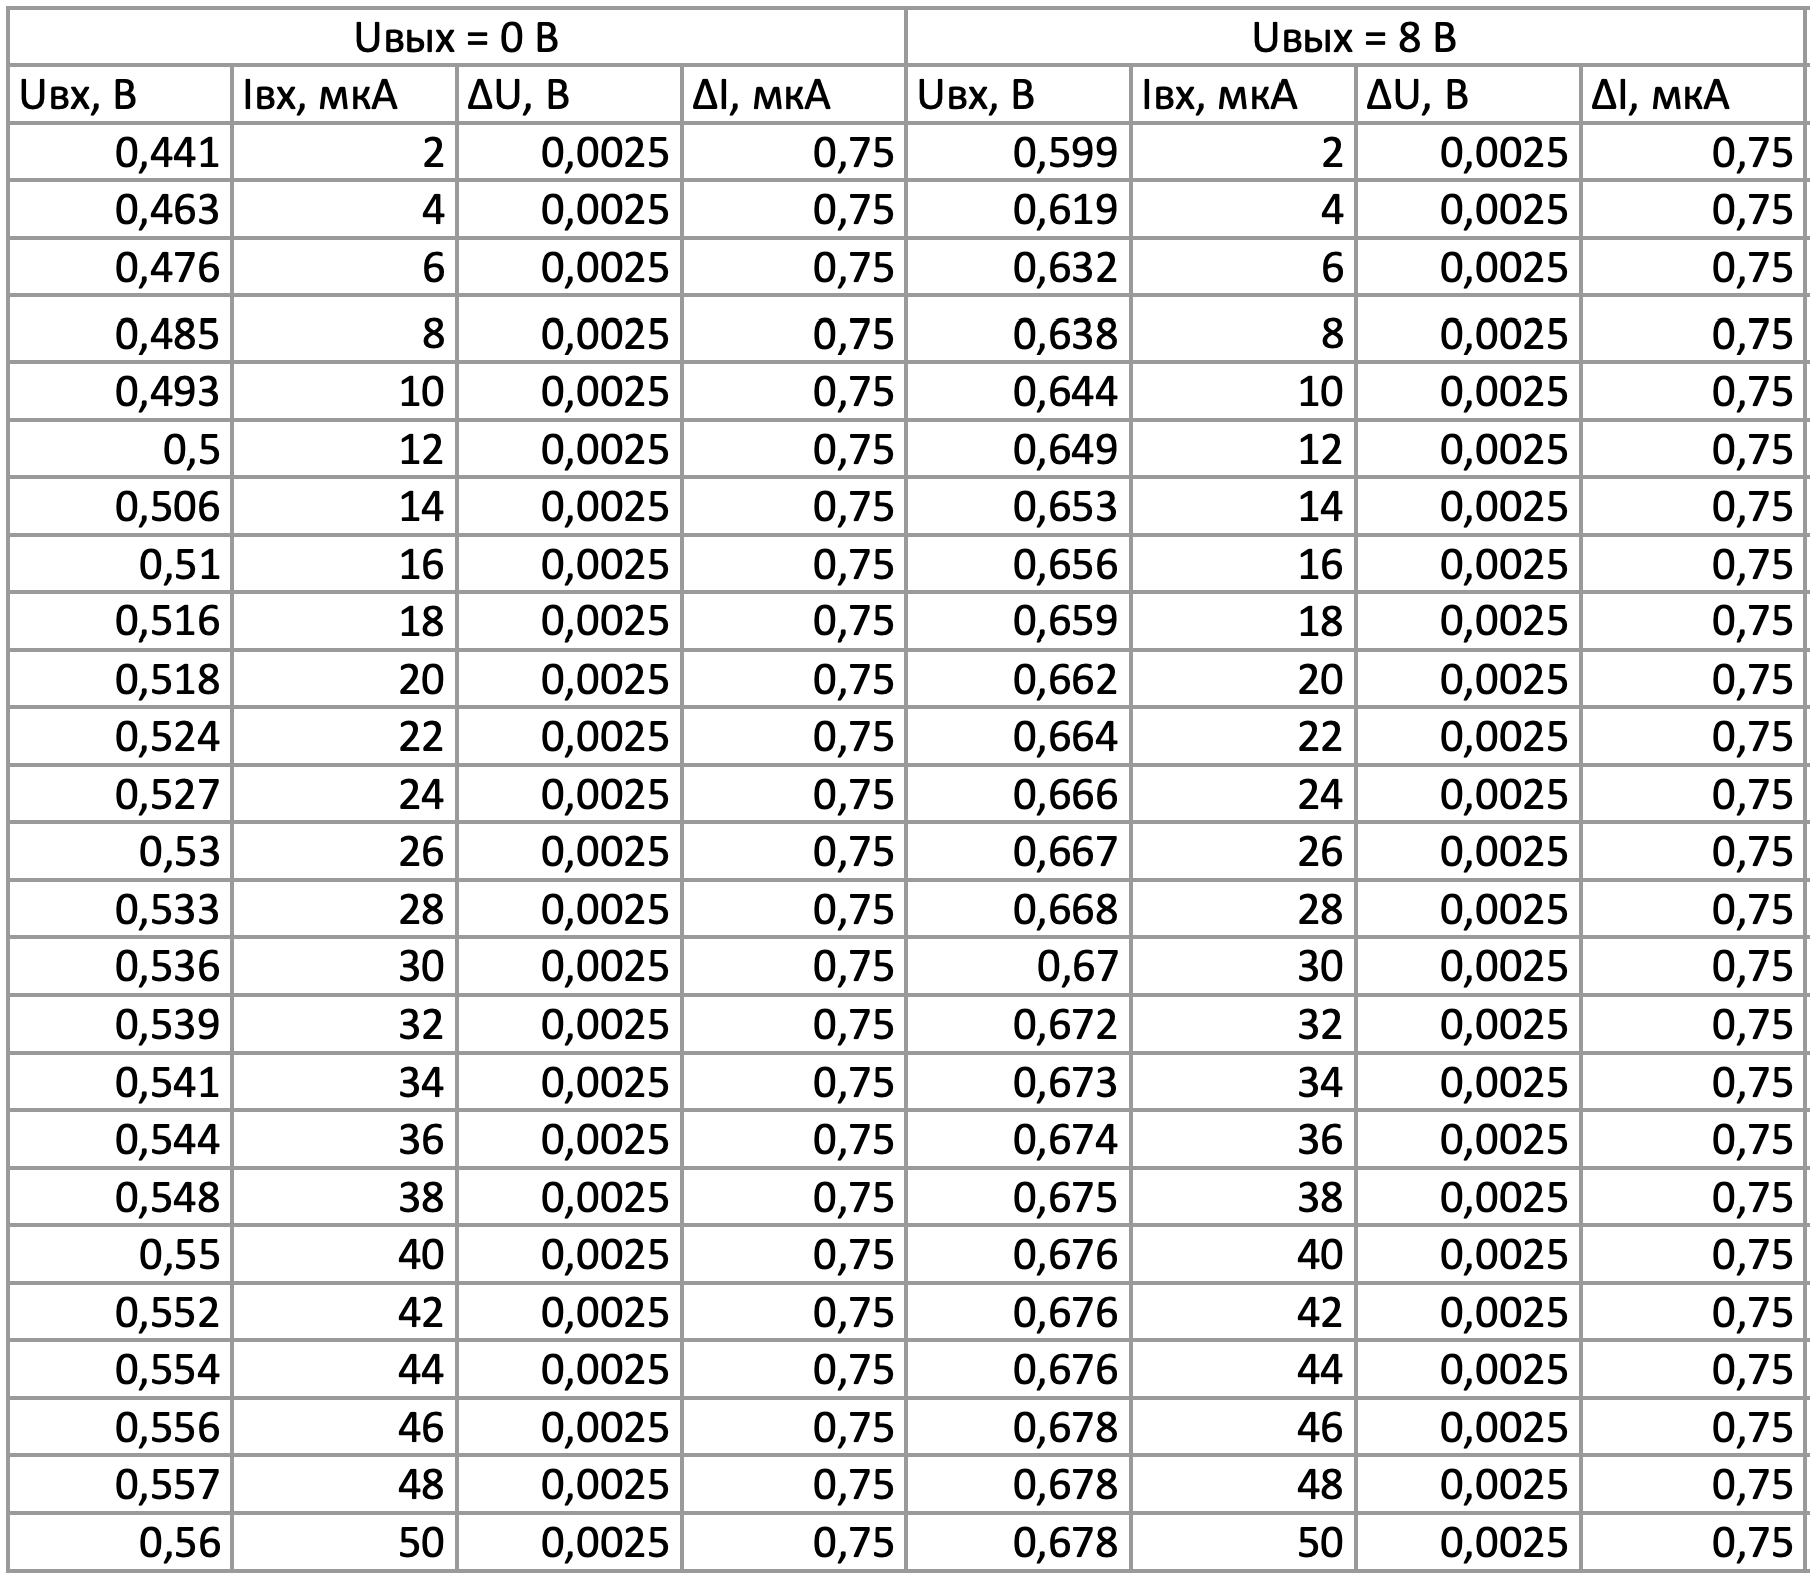
\includegraphics[width=0.9\linewidth]{t_vx.png}}\\
Таб. 1 Значення вхідних струмів та напруг, а також їх похибок при різних напругах виходу.
\end{figure}


\begin{landscape}
\begin{figure}[h]
\center{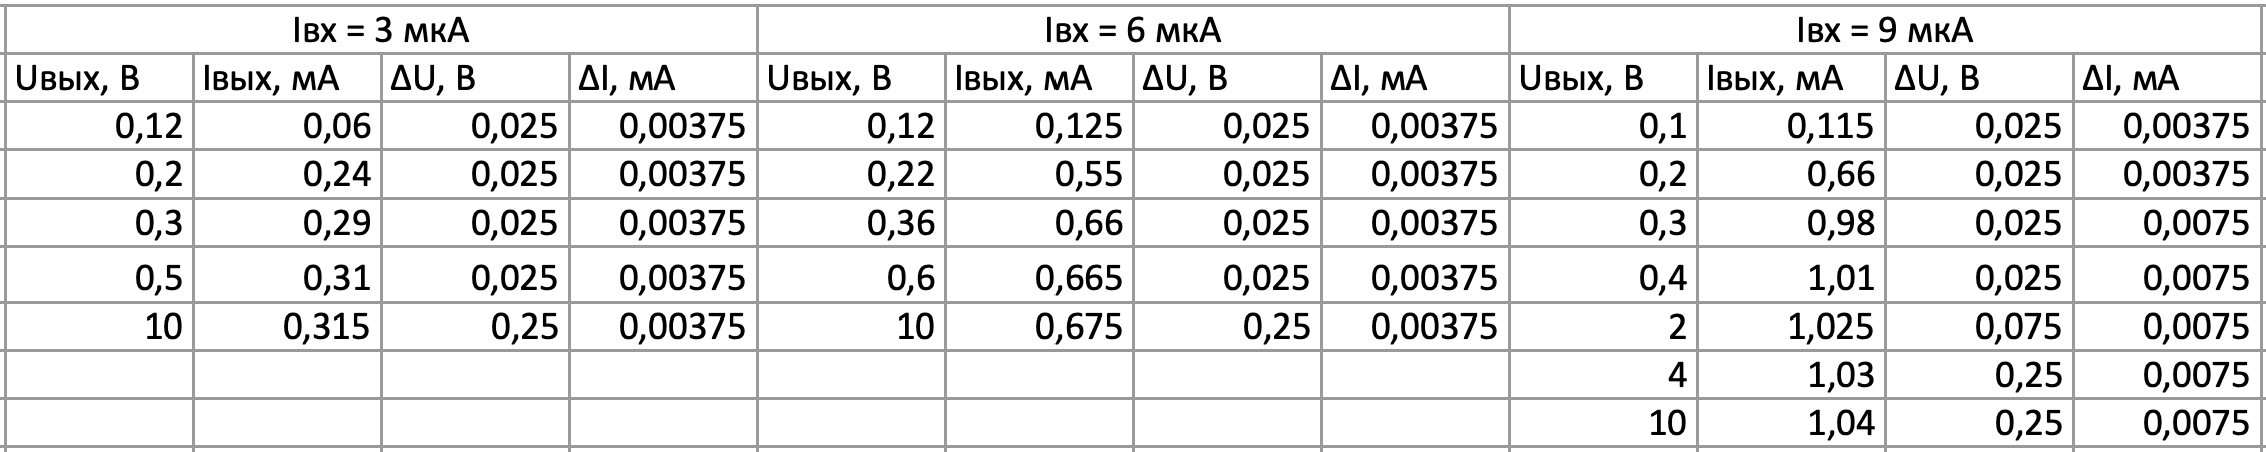
\includegraphics[width=0.9\linewidth]{2.1.png}}
\end{figure}

\begin{figure}[h]
\center{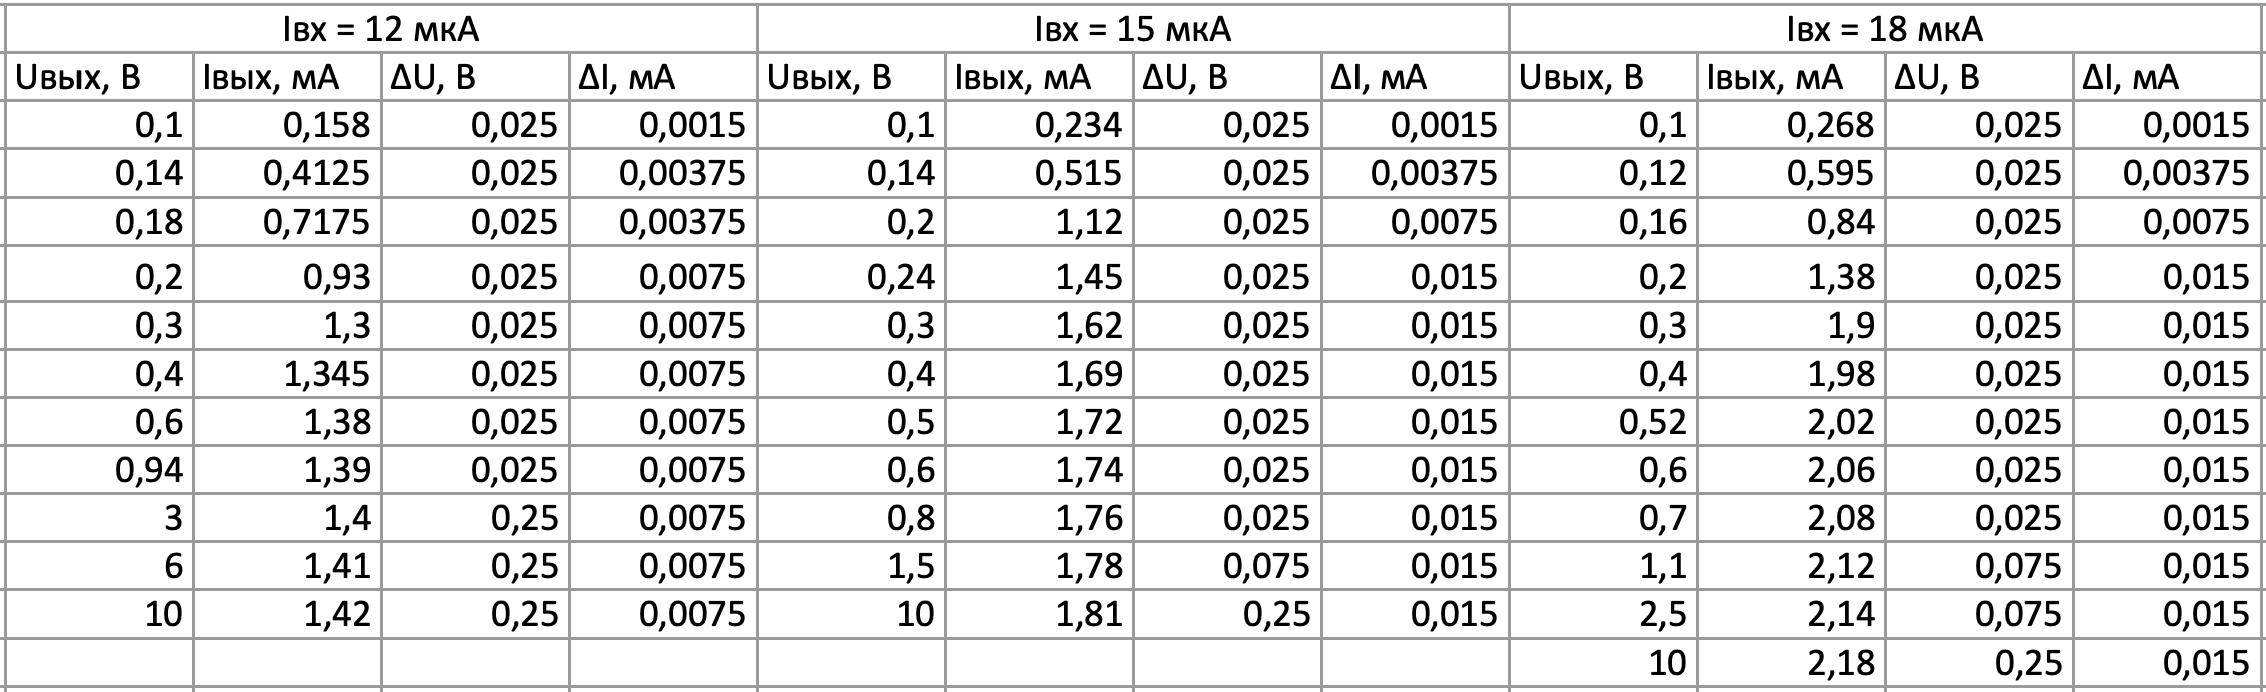
\includegraphics[width=0.9\linewidth]{2.2.png}}
\end{figure}

\begin{figure}[h]
\center{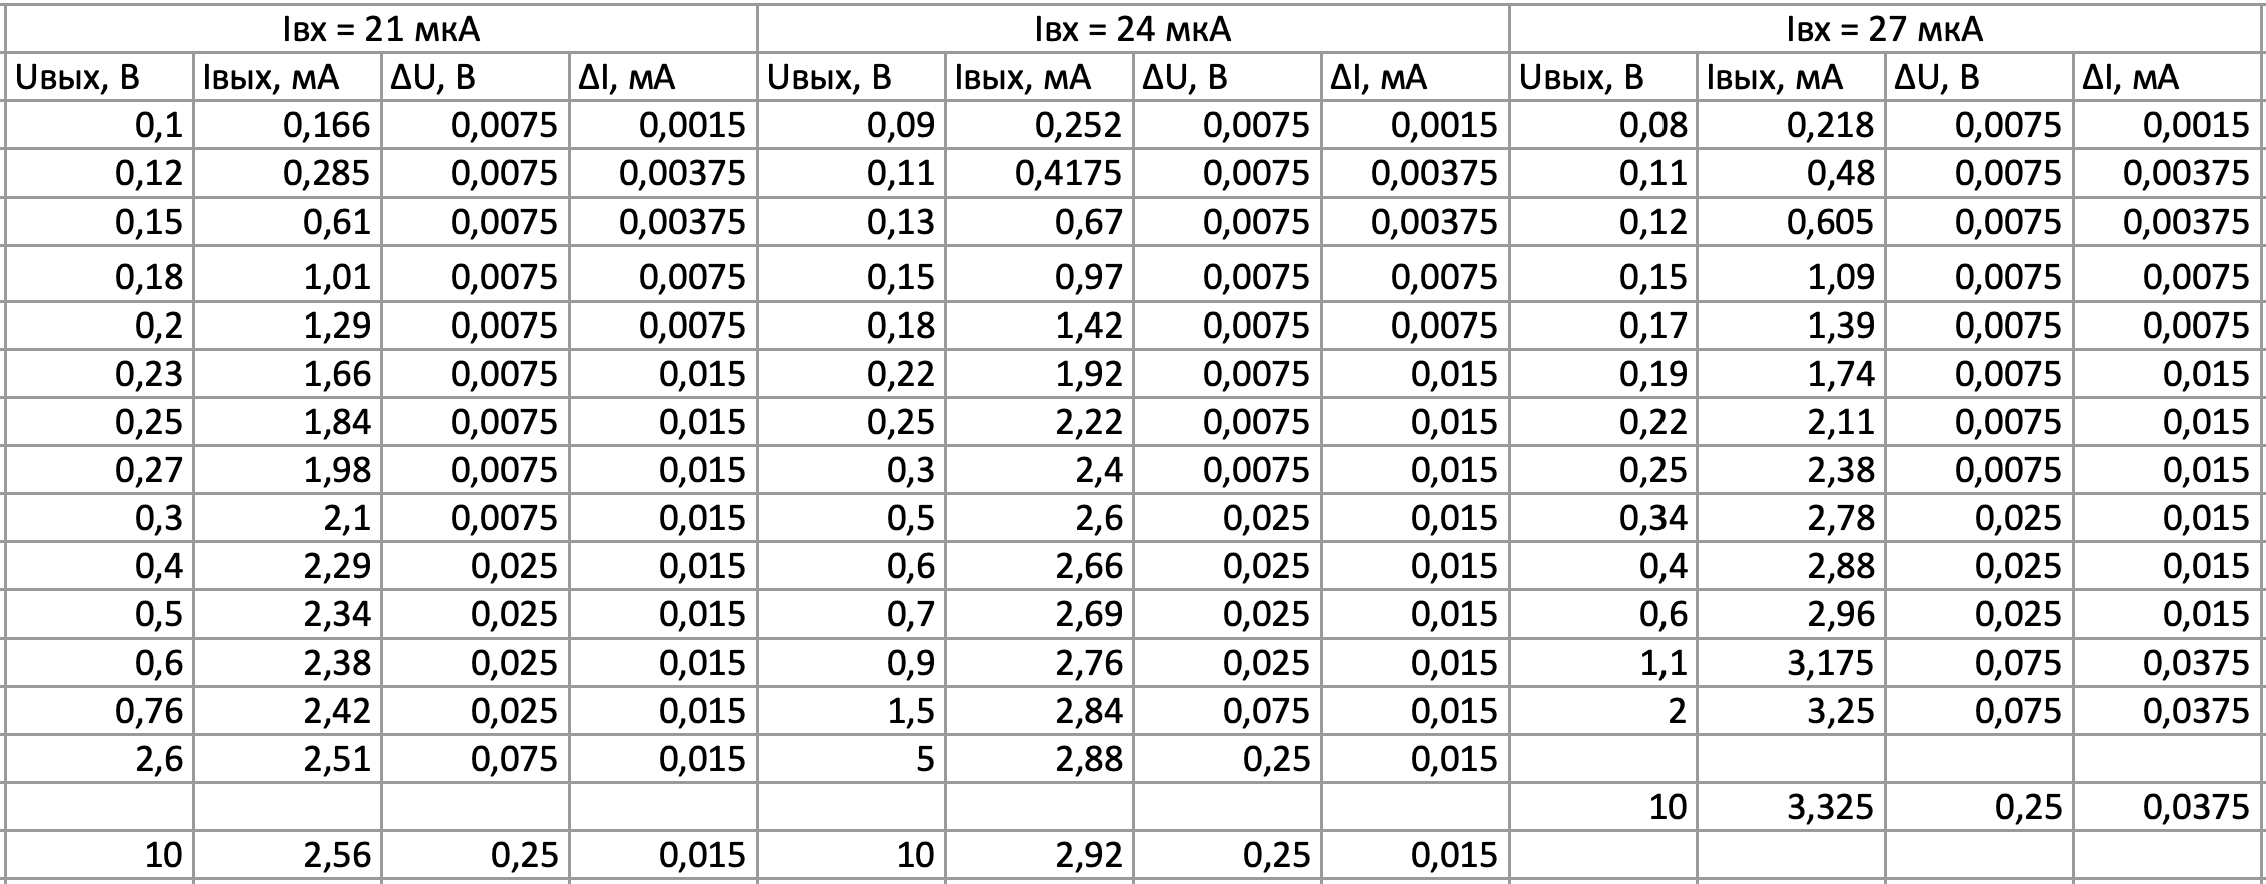
\includegraphics[width=0.9\linewidth]{2.3.png}}
\end{figure}

\begin{figure}[h]
\center{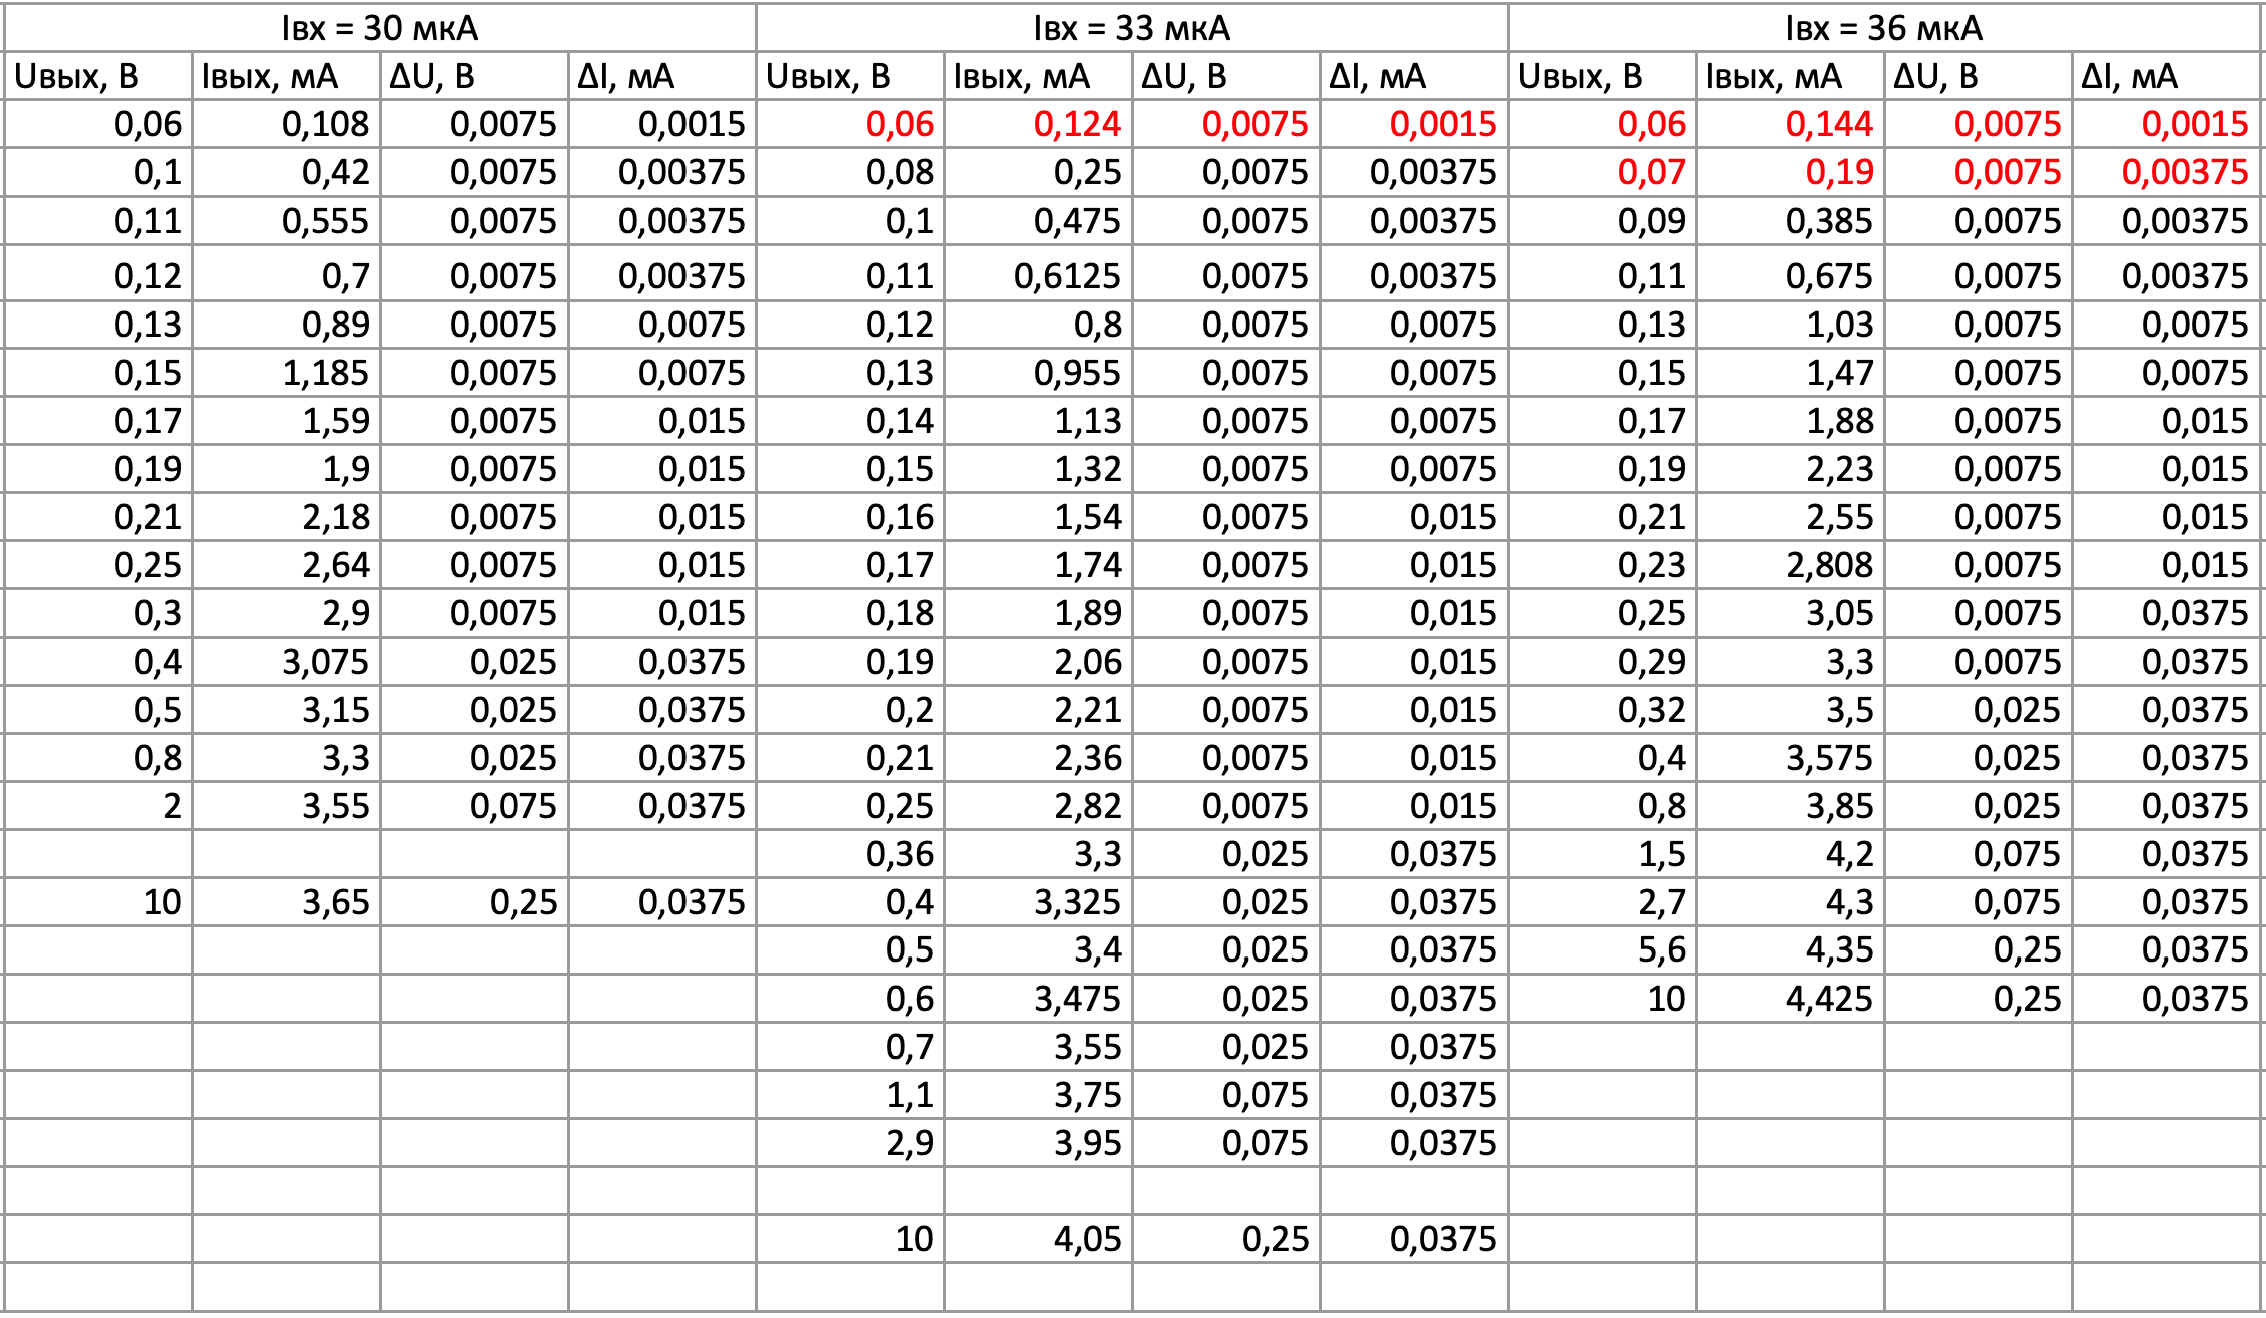
\includegraphics[width=0.9\linewidth]{2.4.png}}
\end{figure}

\begin{figure}[h]
\center{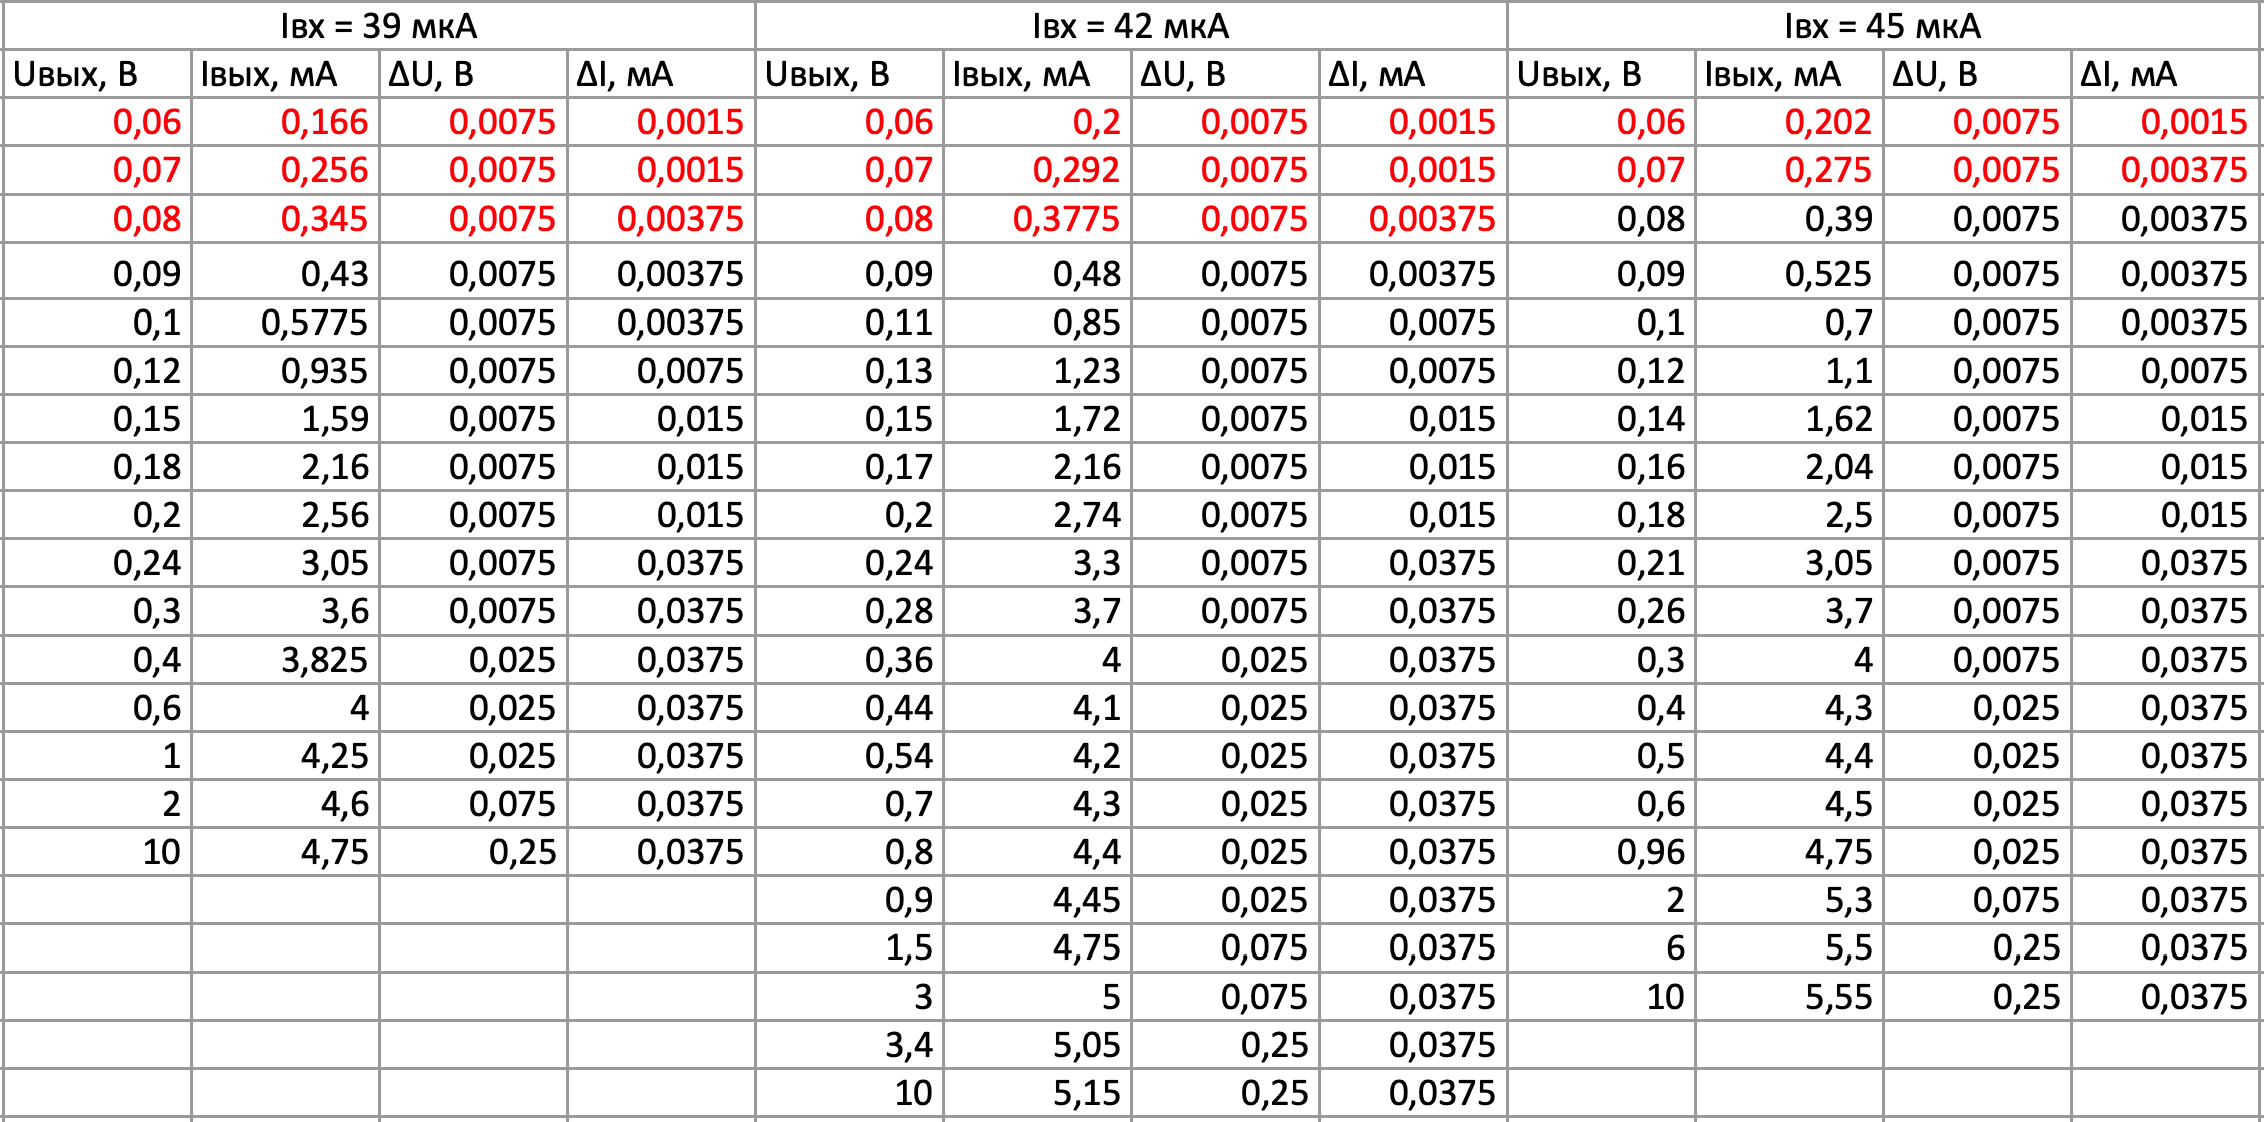
\includegraphics[width=0.9\linewidth]{2.5.png}}\\
Таб. 2 Значення вихідних напруг та струмів, а також їх похибок при різних значеннях вхідного струму.

\end{figure}


\end{landscape}

%-----------------------------------------------------------------------------------------------------------------1----------------------------------------------------------------
\newpage
\begin{center}ГРАФІКИ\\ \end{center}

\begin{figure}[h]
\center{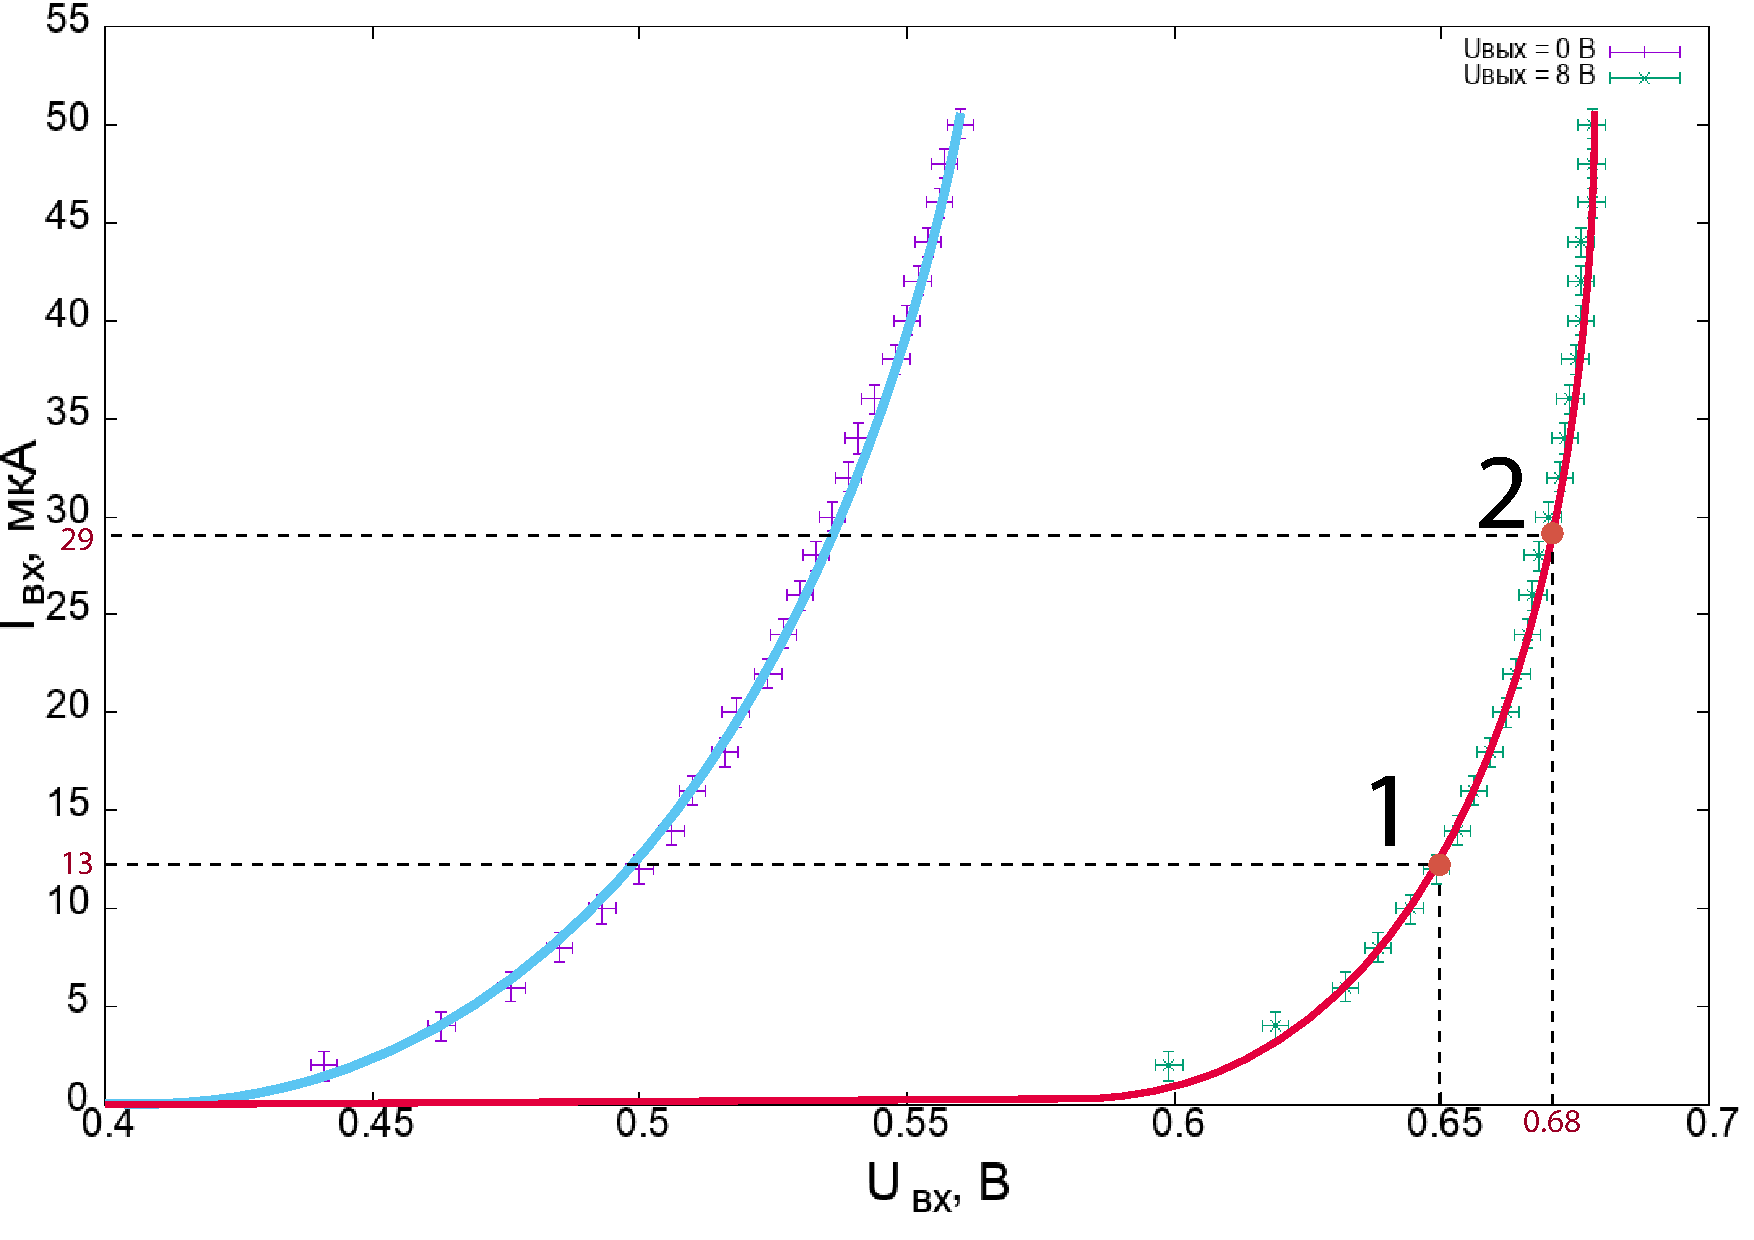
\includegraphics[width=0.9\linewidth]{1.pdf}}
\caption{Сімейство вхідних характеристик транзистора.}
\label{ris:image5}
\end{figure}
Опір на емітері визачається формулою:
\begin{equation}\label{eq1}
R_{\text{вх}} = \dfrac{\triangle U_{\text{ЕБ}}}{\triangle I_{\text{Б}}}
\end{equation}


Оскільки в нас є $\triangle I$ та $\triangle U$ то можна обрати двi робочi точки 1 та 2, які лежать на однiй кривiй, а саме кривій яка відповідає напрузі колектор-емiтер. Оскьльки точки 1 та 2 мають дві координати (позначимо їх як 1($U_{\text{ЕБ$_1$}}, I_{\text{Б$_1$}})$ та 1($U_{\text{ЕБ$_2$}}, I_{\text{Б$_2$}}$)) і використовуючи формулу (\ref{eq1}) можна записати вираз:

\begin{equation}\label{eq2}
R_{\text{вх}} = \dfrac{U_{\text{ЕБ$_2$}} - U_{\text{ЕБ$_1$}}}{ I_{\text{Б$_2$}} -  I_{\text{Б$_1$}}}
\end{equation}
підставляючи отримаємо, що
\begin{equation}\label{eq3}
R_{\text{вх}} = 625 \text{ Ом}
\end{equation}
Також з цього графіка можна знайти $I_{\text{б}}$ взявши середн'є значення між 1 та 2 точкою і провевши перпендикуляр на вісь Y, отримаю $I_{\text{б}} \approx 20  \text{ мкА}$.

%-----------------------------------------------------------------------------------------------------------------2----------------------------------------------------------------
\newpage
Використовуючи формулу (\ref{eq4}) та рис. \ref{ris:image5} знайду тобто опір виходу.

\begin{equation}\label{eq4}
R_{\text{вих}} = \dfrac{\triangle U_{\text{ЕК}}}{\triangle I_{\text{К}}}
\end{equation}

\begin{figure}[h]
\center{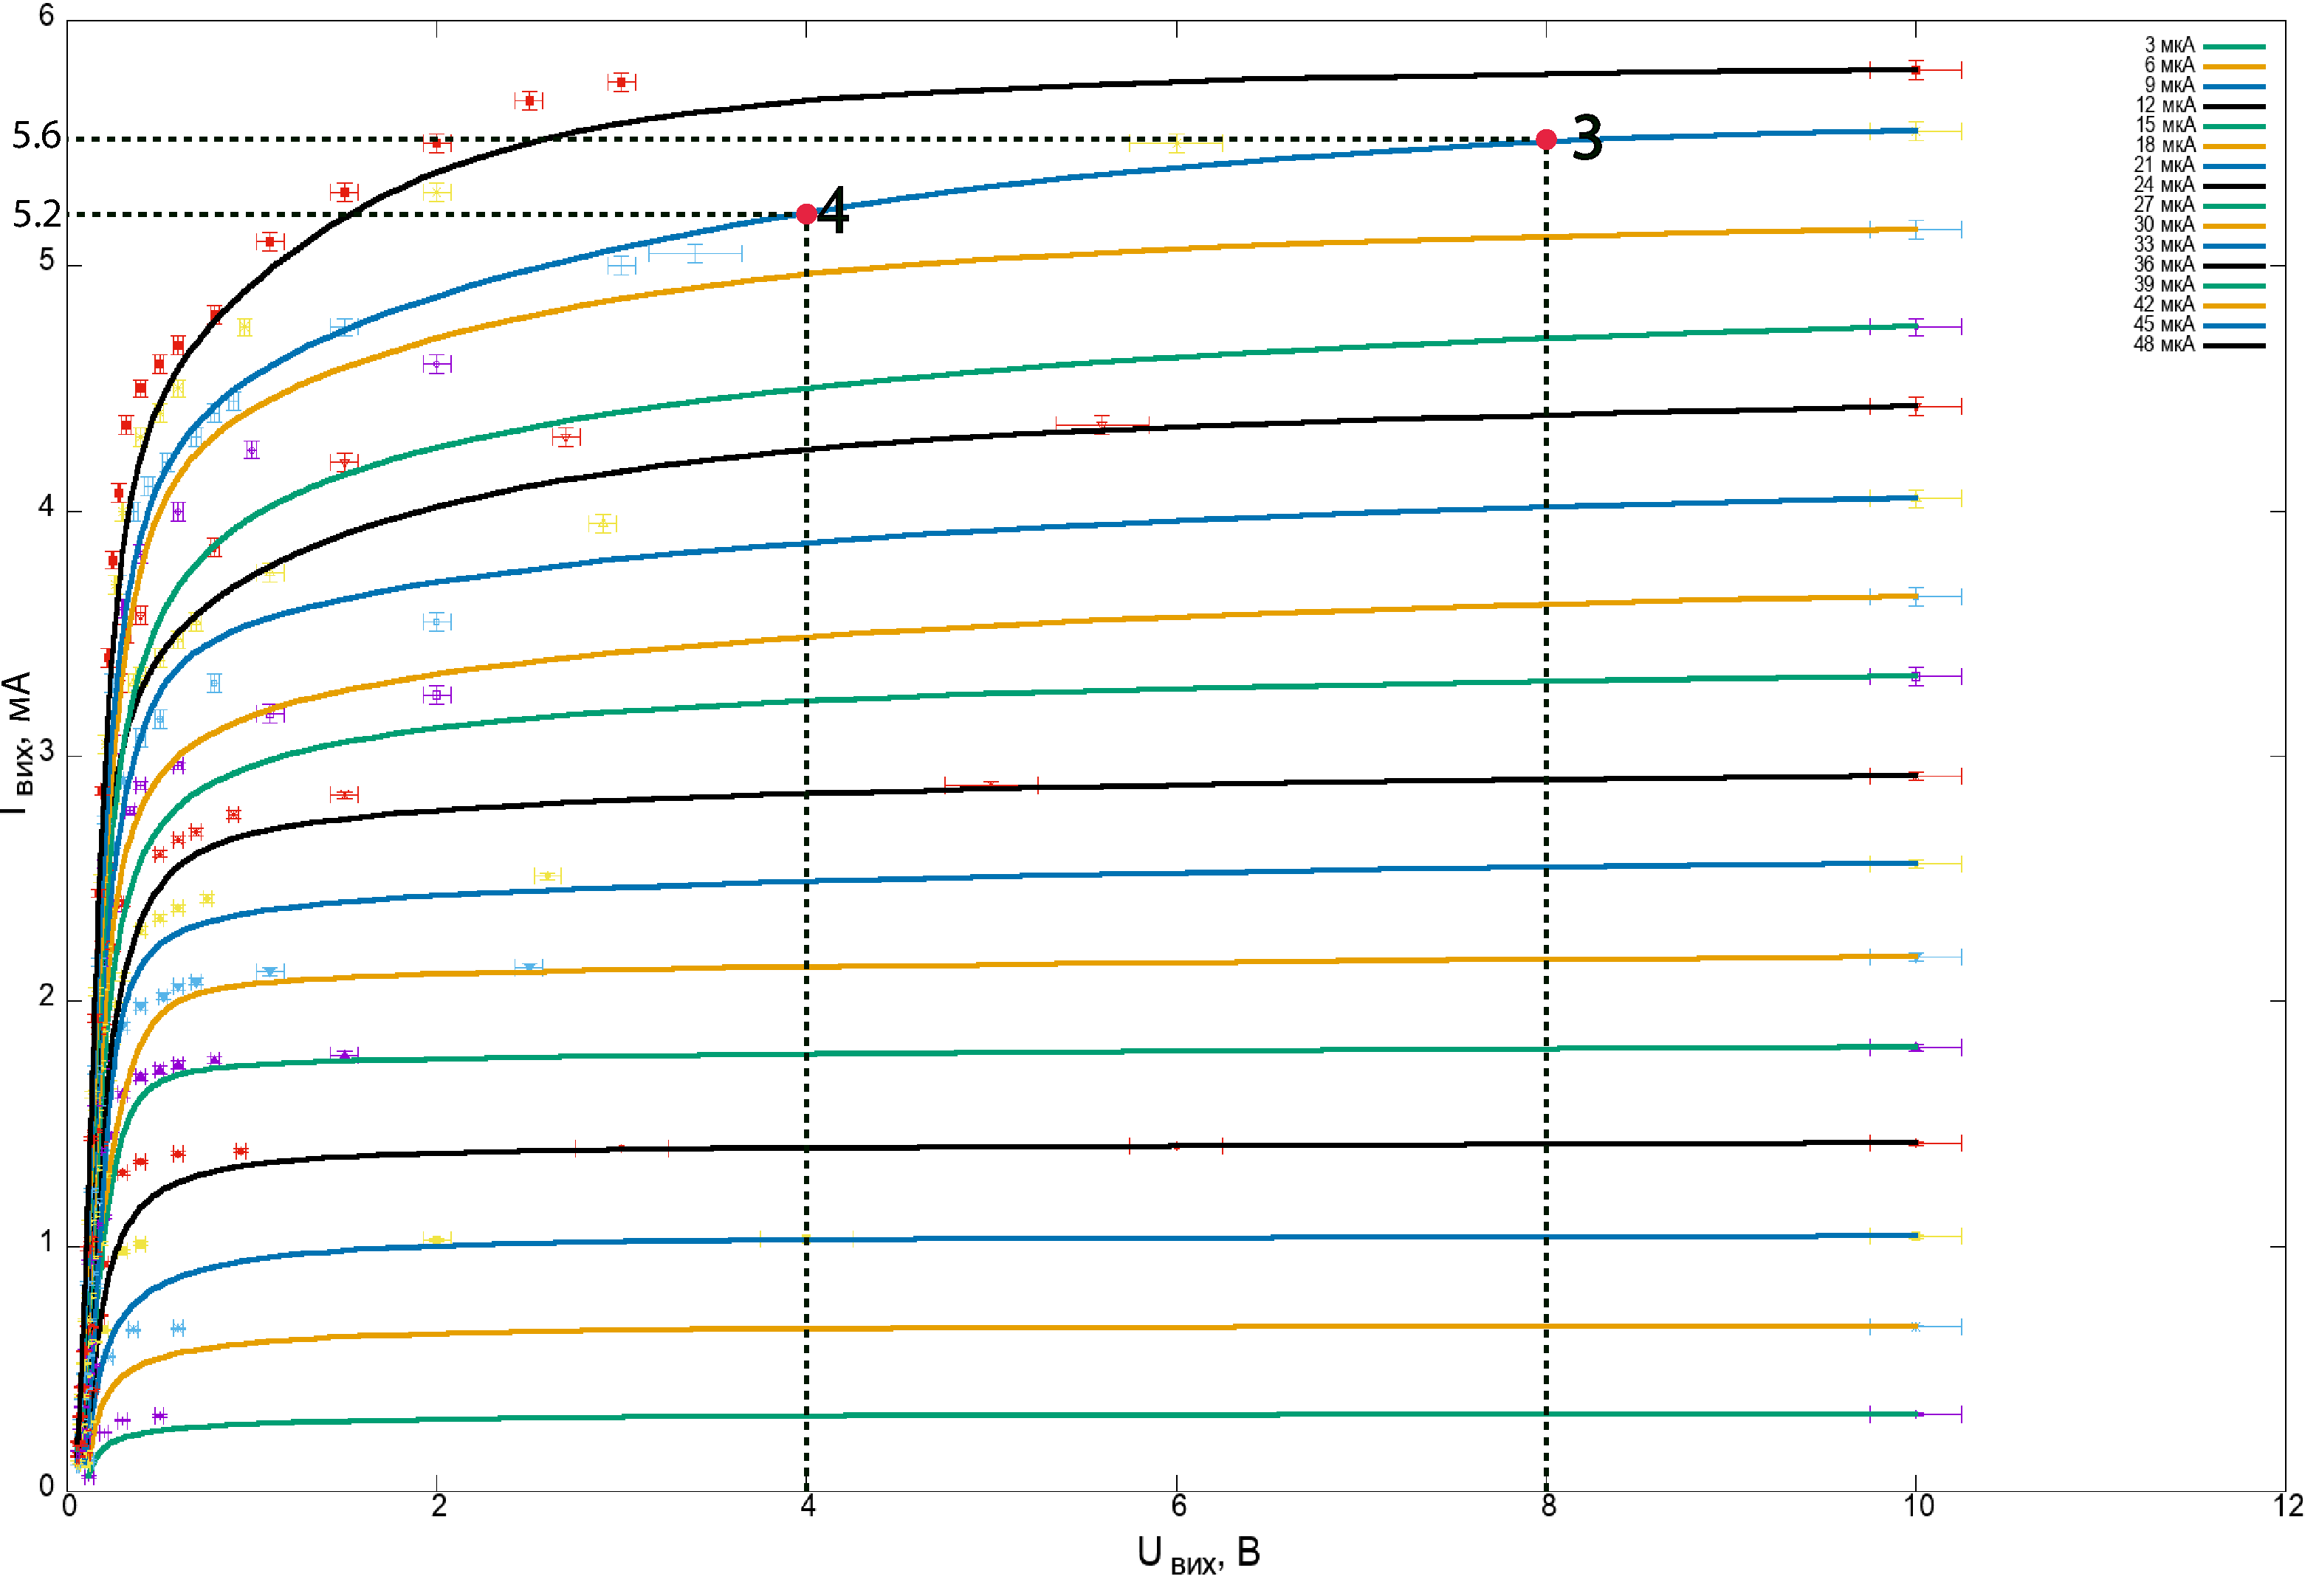
\includegraphics[width=0.9\linewidth]{2.pdf}}
\caption{Сімейство вихідних характеристик транзистора.}
\label{ris:image5}
\end{figure}


Аналогічно з вхiдними характеристиками можна обрати на рис. \ref{ris:image5}
 робочу точку 3, таким чином, щоб перпендикуляр, опущений з неї на вiсь Х, був на 8 В, оскiльки на вхiдних характеристиках ця сама робоча точка 1 розташовувалась на гiлцi, що вiдповiдала напрузi U. \\
Зважаючи на те що $I_{\text{Б}} = const$, тоді точки 3 і 4 розташоую на одніий кривій, але таким чином щоб була помітна різниця у значеннях.
Виконую аналогічні операції і знаходжу:\\
 $R_{\text{вих}}$
\begin{equation}\label{eq5}
R_{\text{вих}} = \dfrac{U_{\text{ЕК$_2$}} - U_{\text{ЕК$_1$}}}{ I_{\text{К$_2$}} - I_{\text{К$_1$}}} = 12,6 \text{ кОм}
\end{equation}
Взявши середнє значення між точками C та D можна знайти $I_{\text{К}}\approx 5,46$

Знаючи струм бази та струм колектора, можу знайти струм емiтера, використовуючи формулу для коефiцiєнта пiдсилення за струмом для спiльного емiтера наступним чином:
\begin{equation}\label{eq6}
\beta = \dfrac{I_{\text{К}}}{I_{\text{Б}}} =  \dfrac{I_{\text{К}}}{I_{\text{Е}} - I_{\text{К}}} \Rightarrow I_{\text{Е}} = I_{\text{Б}} + I_{\text{К}} = 0,02\cdot 10^{-3} + 5,46 \cdot 10^{-3} = 5,48 \text{мА}
\end{equation}

%------------------------------------------------------------------------------------------3--------------------------------------------------------------------------------------
\newpage
Коефiцiєнт пiдсилення за струмом для спiльного емiтера знаходжу так:
\begin{equation}\label{eq7}
\beta = \dfrac{5,46}{0,02} = 273
\end{equation}

Коеф. пiдсилення струму бази:
\begin{equation}\label{eq8}
\alpha = \dfrac{I_{\text{К}}}{I_{\text{Е}}} =  \dfrac{5,46}{5,48}\approx 0,99
\end{equation}

Знаючи струм емiтера, можна знайти опiр емiтера за наступною формулою:
\begin{equation}\label{eq9}
r_\text{Е} = \dfrac{\varphi_T}{I_\text{Е}}= \dfrac{27}{5,46} \approx 4,9  \text{ Ом}
\end{equation}

Для того щоб визначити дифузiйний потенцiал емiтерного переходу  $\varphi_0$ проводжу дотичну до точки, що знаходиться посерединi мiж  1 та 2 точкою і отримаю наступне:
\begin{figure}[h!]
\center{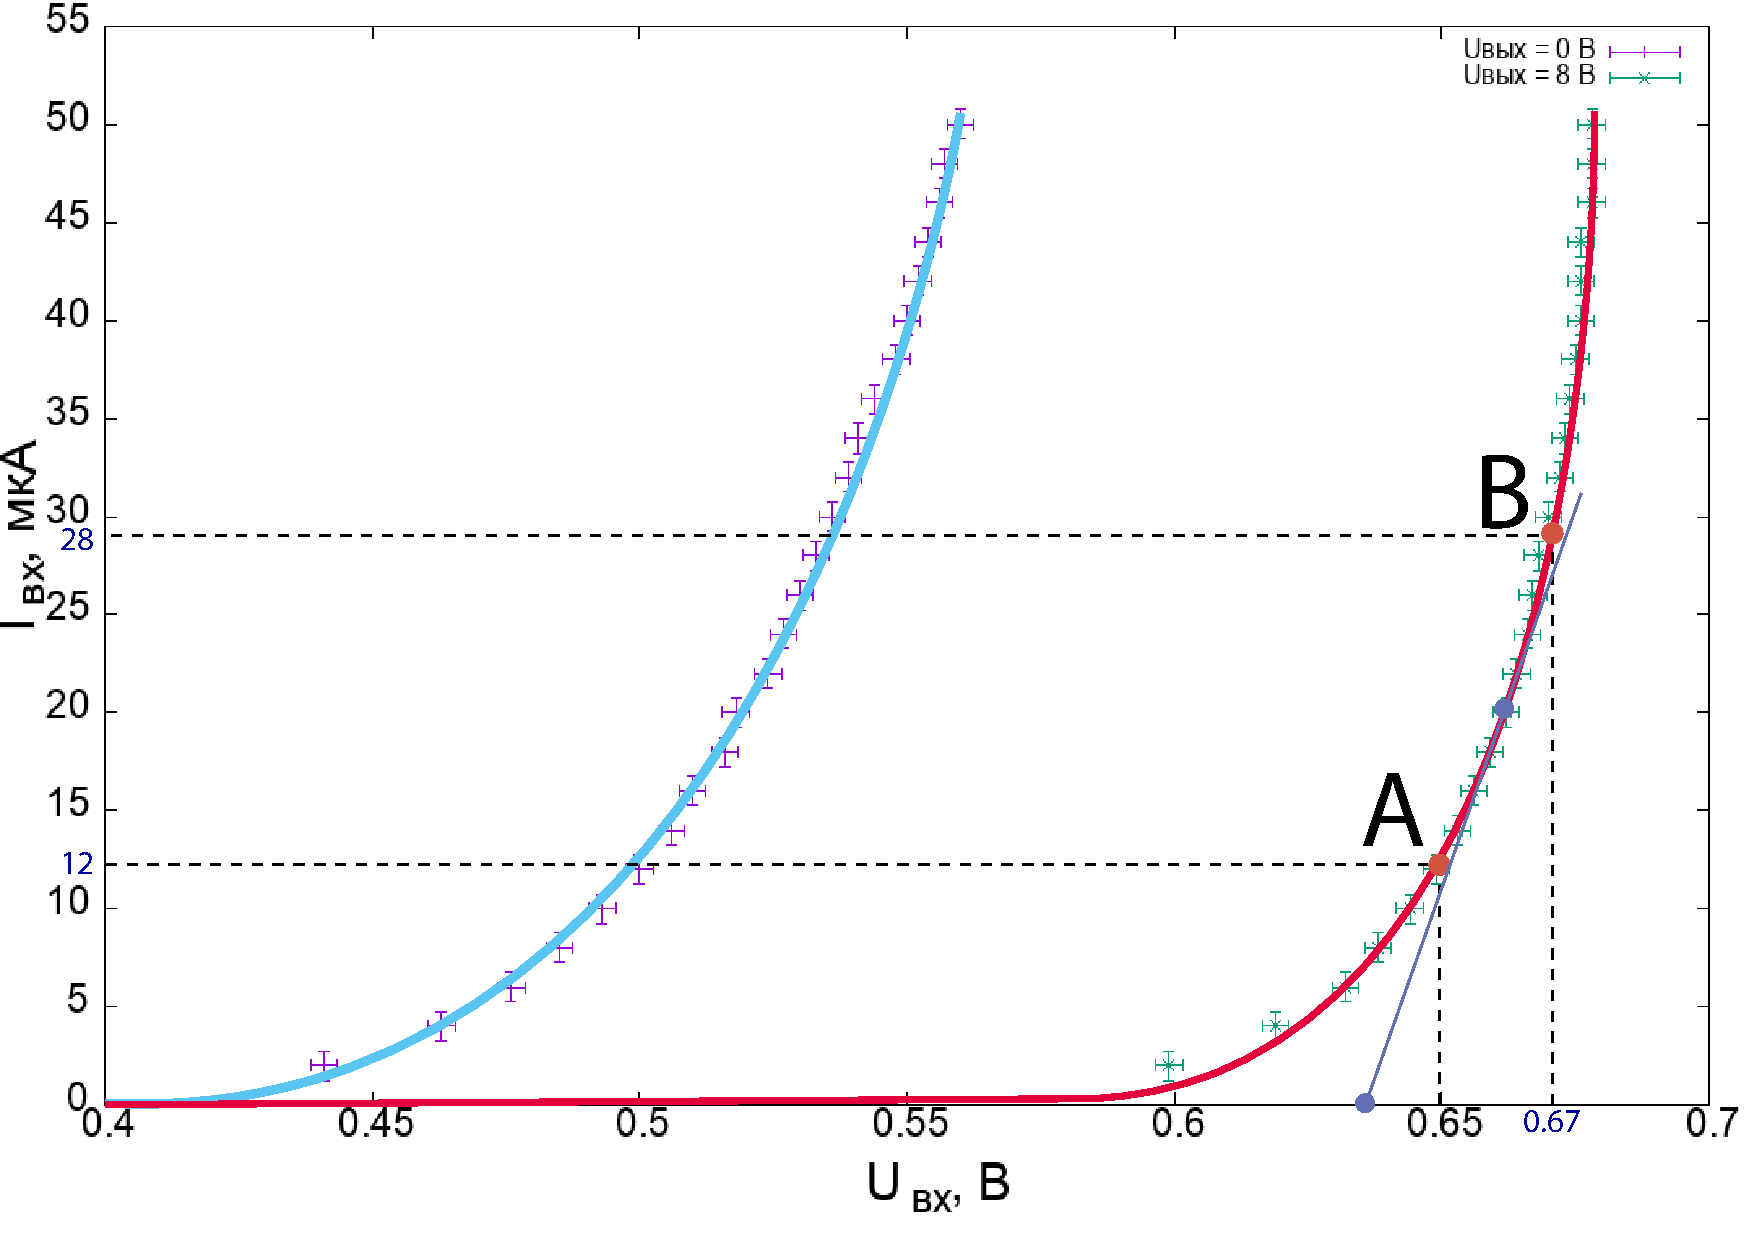
\includegraphics[width=0.9\linewidth]{1.1.pdf}}
\caption{Графічне визначення дифузiйного потенцiау емiтерного переходу.}
\label{ris:image9}
\end{figure}

\begin{equation}\label{eq10}
\varphi_0 = 0,6373  \text {В}
\end{equation}

 Знаючи струм бази та дифузiйний потенцiал, тепер можна і опiр бази знайти:
\begin{equation}\label{eq11}
r_\text{Б} = \dfrac{\varphi_0}{I_\text{Б}} =  \dfrac{0,6373}{0,02 \cdot 10^{-3}}  \approx 32  \text{ кОм}
\end{equation}






%---------------------------------------------------------------------------------------------------------------------------------------------------------------------------------
\clearpage
\newpage
\begin{center}Висновки\\ \end{center}
В даній лабораторній роботі я провела дослідження біполярного транзистора, побудувала сiмейство вихiдних та вхідних характеристик транзистора за вхідними значеннями. На основі аналізу вхідних і вихідних характеристик, можна сказати, що під час зняття результатів дослідження
сімейства характеристик транзистор був підключений у схему з загальним
емітером,про це свідчить вихідні характеристики, оскільки там перетин перетинає вісь X а не Y як у схемі з загальною базою.




















\end{document}
